\documentclass[1p]{elsarticle_modified}
%\bibliographystyle{elsarticle-num}

%\usepackage[colorlinks]{hyperref}
%\usepackage{abbrmath_seonhwa} %\Abb, \Ascr, \Acal ,\Abf, \Afrak
\usepackage{amsfonts}
\usepackage{amssymb}
\usepackage{amsmath}
\usepackage{amsthm}
\usepackage{scalefnt}
\usepackage{amsbsy}
\usepackage{kotex}
\usepackage{caption}
\usepackage{subfig}
\usepackage{color}
\usepackage{graphicx}
\usepackage{xcolor} %% white, black, red, green, blue, cyan, magenta, yellow
\usepackage{float}
\usepackage{setspace}
\usepackage{hyperref}

\usepackage{tikz}
\usetikzlibrary{arrows}

\usepackage{multirow}
\usepackage{array} % fixed length table
\usepackage{hhline}

%%%%%%%%%%%%%%%%%%%%%
\makeatletter
\renewcommand*\env@matrix[1][\arraystretch]{%
	\edef\arraystretch{#1}%
	\hskip -\arraycolsep
	\let\@ifnextchar\new@ifnextchar
	\array{*\c@MaxMatrixCols c}}
\makeatother %https://tex.stackexchange.com/questions/14071/how-can-i-increase-the-line-spacing-in-a-matrix
%%%%%%%%%%%%%%%

\usepackage[normalem]{ulem}

\newcommand{\msout}[1]{\ifmmode\text{\sout{\ensuremath{#1}}}\else\sout{#1}\fi}
%SOURCE: \msout is \stkout macro in https://tex.stackexchange.com/questions/20609/strikeout-in-math-mode

\newcommand{\cancel}[1]{
	\ifmmode
	{\color{red}\msout{#1}}
	\else
	{\color{red}\sout{#1}}
	\fi
}

\newcommand{\add}[1]{
	{\color{blue}\uwave{#1}}
}

\newcommand{\replace}[2]{
	\ifmmode
	{\color{red}\msout{#1}}{\color{blue}\uwave{#2}}
	\else
	{\color{red}\sout{#1}}{\color{blue}\uwave{#2}}
	\fi
}

\newcommand{\Sol}{\mathcal{S}} %segment
\newcommand{\D}{D} %diagram
\newcommand{\A}{\mathcal{A}} %arc


%%%%%%%%%%%%%%%%%%%%%%%%%%%%%5 test

\def\sl{\operatorname{\textup{SL}}(2,\Cbb)}
\def\psl{\operatorname{\textup{PSL}}(2,\Cbb)}
\def\quan{\mkern 1mu \triangleright \mkern 1mu}

\theoremstyle{definition}
\newtheorem{thm}{Theorem}[section]
\newtheorem{prop}[thm]{Proposition}
\newtheorem{lem}[thm]{Lemma}
\newtheorem{ques}[thm]{Question}
\newtheorem{cor}[thm]{Corollary}
\newtheorem{defn}[thm]{Definition}
\newtheorem{exam}[thm]{Example}
\newtheorem{rmk}[thm]{Remark}
\newtheorem{alg}[thm]{Algorithm}

\newcommand{\I}{\sqrt{-1}}
\begin{document}

%\begin{frontmatter}
%
%\title{Boundary parabolic representations of knots up to 8 crossings}
%
%%% Group authors per affiliation:
%\author{Yunhi Cho} 
%\address{Department of Mathematics, University of Seoul, Seoul, Korea}
%\ead{yhcho@uos.ac.kr}
%
%
%\author{Seonhwa Kim} %\fnref{s_kim}}
%\address{Center for Geometry and Physics, Institute for Basic Science, Pohang, 37673, Korea}
%\ead{ryeona17@ibs.re.kr}
%
%\author{Hyuk Kim}
%\address{Department of Mathematical Sciences, Seoul National University, Seoul 08826, Korea}
%\ead{hyukkim@snu.ac.kr}
%
%\author{Seokbeom Yoon}
%\address{Department of Mathematical Sciences, Seoul National University, Seoul, 08826,  Korea}
%\ead{sbyoon15@snu.ac.kr}
%
%\begin{abstract}
%We find all boundary parabolic representation of knots up to 8 crossings.
%
%\end{abstract}
%\begin{keyword}
%    \MSC[2010] 57M25 
%\end{keyword}
%
%\end{frontmatter}

%\linenumbers
%\tableofcontents
%
\newcommand\colored[1]{\textcolor{white}{\rule[-0.35ex]{0.8em}{1.4ex}}\kern-0.8em\color{red} #1}%
%\newcommand\colored[1]{\textcolor{white}{ #1}\kern-2.17ex	\textcolor{white}{ #1}\kern-1.81ex	\textcolor{white}{ #1}\kern-2.15ex\color{red}#1	}

{\Large $\underline{12a_{0676}~(K12a_{0676})}$}

\setlength{\tabcolsep}{10pt}
\renewcommand{\arraystretch}{1.6}
\vspace{1cm}\begin{tabular}{m{100pt}>{\centering\arraybackslash}m{274pt}}
\multirow{5}{120pt}{
	\centering
	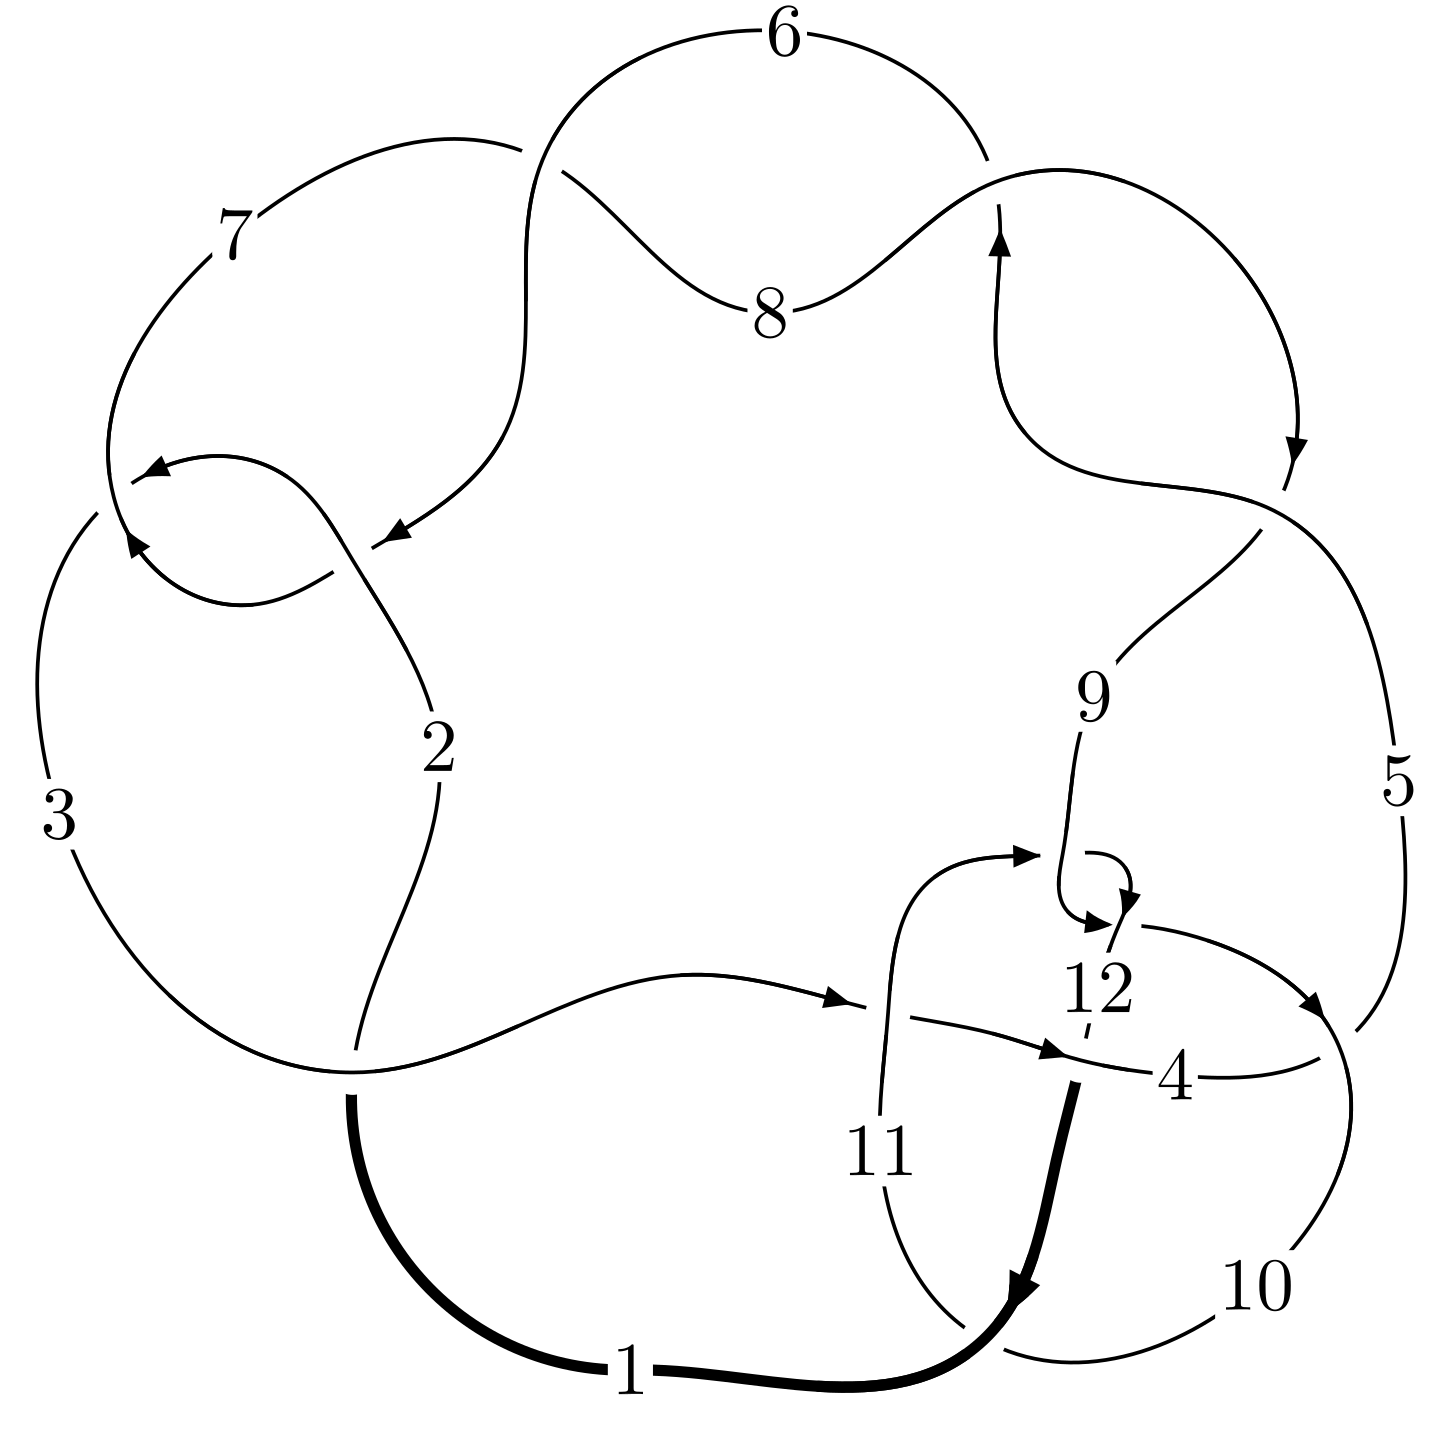
\includegraphics[width=112pt]{../../../GIT/diagram.site/Diagrams/png/1477_12a_0676.png}\\
\ \ \ A knot diagram\footnotemark}&
\allowdisplaybreaks
\textbf{Linearized knot diagam} \\
\cline{2-2}
 &
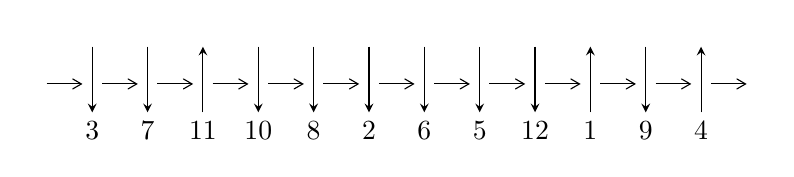
\begin{tikzpicture}[x=20pt, y=17pt]
	% nodes
	\node (C0) at (0, 0) {};
	\node (C1) at (1, 0) {};
	\node (C1U) at (1, +1) {};
	\node (C1D) at (1, -1) {3};

	\node (C2) at (2, 0) {};
	\node (C2U) at (2, +1) {};
	\node (C2D) at (2, -1) {7};

	\node (C3) at (3, 0) {};
	\node (C3U) at (3, +1) {};
	\node (C3D) at (3, -1) {11};

	\node (C4) at (4, 0) {};
	\node (C4U) at (4, +1) {};
	\node (C4D) at (4, -1) {10};

	\node (C5) at (5, 0) {};
	\node (C5U) at (5, +1) {};
	\node (C5D) at (5, -1) {8};

	\node (C6) at (6, 0) {};
	\node (C6U) at (6, +1) {};
	\node (C6D) at (6, -1) {2};

	\node (C7) at (7, 0) {};
	\node (C7U) at (7, +1) {};
	\node (C7D) at (7, -1) {6};

	\node (C8) at (8, 0) {};
	\node (C8U) at (8, +1) {};
	\node (C8D) at (8, -1) {5};

	\node (C9) at (9, 0) {};
	\node (C9U) at (9, +1) {};
	\node (C9D) at (9, -1) {12};

	\node (C10) at (10, 0) {};
	\node (C10U) at (10, +1) {};
	\node (C10D) at (10, -1) {1};

	\node (C11) at (11, 0) {};
	\node (C11U) at (11, +1) {};
	\node (C11D) at (11, -1) {9};

	\node (C12) at (12, 0) {};
	\node (C12U) at (12, +1) {};
	\node (C12D) at (12, -1) {4};
	\node (C13) at (13, 0) {};

	% arrows
	\draw[->,>={angle 60}]
	(C0) edge (C1) (C1) edge (C2) (C2) edge (C3) (C3) edge (C4) (C4) edge (C5) (C5) edge (C6) (C6) edge (C7) (C7) edge (C8) (C8) edge (C9) (C9) edge (C10) (C10) edge (C11) (C11) edge (C12) (C12) edge (C13) ;	\draw[->,>=stealth]
	(C1U) edge (C1D) (C2U) edge (C2D) (C3D) edge (C3U) (C4U) edge (C4D) (C5U) edge (C5D) (C6U) edge (C6D) (C7U) edge (C7D) (C8U) edge (C8D) (C9U) edge (C9D) (C10D) edge (C10U) (C11U) edge (C11D) (C12D) edge (C12U) ;
	\end{tikzpicture} \\
\hhline{~~} \\& 
\textbf{Solving Sequence} \\ \cline{2-2} 
 &
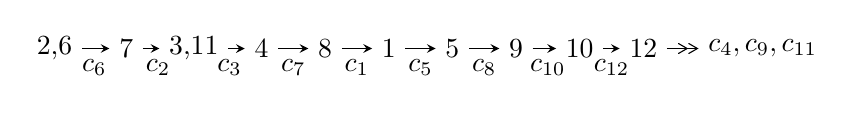
\begin{tikzpicture}[x=23pt, y=7pt]
	% node
	\node (A0) at (-1/8, 0) {2,6};
	\node (A1) at (1, 0) {7};
	\node (A2) at (33/16, 0) {3,11};
	\node (A3) at (25/8, 0) {4};
	\node (A4) at (33/8, 0) {8};
	\node (A5) at (41/8, 0) {1};
	\node (A6) at (49/8, 0) {5};
	\node (A7) at (57/8, 0) {9};
	\node (A8) at (65/8, 0) {10};
	\node (A9) at (73/8, 0) {12};
	\node (C1) at (1/2, -1) {$c_{6}$};
	\node (C2) at (3/2, -1) {$c_{2}$};
	\node (C3) at (21/8, -1) {$c_{3}$};
	\node (C4) at (29/8, -1) {$c_{7}$};
	\node (C5) at (37/8, -1) {$c_{1}$};
	\node (C6) at (45/8, -1) {$c_{5}$};
	\node (C7) at (53/8, -1) {$c_{8}$};
	\node (C8) at (61/8, -1) {$c_{10}$};
	\node (C9) at (69/8, -1) {$c_{12}$};
	\node (A10) at (11, 0) {$c_{4},c_{9},c_{11}$};

	% edge
	\draw[->,>=stealth]	
	(A0) edge (A1) (A1) edge (A2) (A2) edge (A3) (A3) edge (A4) (A4) edge (A5) (A5) edge (A6) (A6) edge (A7) (A7) edge (A8) (A8) edge (A9) ;
	\draw[->>,>={angle 60}]	
	(A9) edge (A10);
\end{tikzpicture} \\ 

\end{tabular} \\

\footnotetext{
The image of knot diagram is generated by the software ``\textbf{Draw programme}" developed by Andrew Bartholomew(\url{http://www.layer8.co.uk/maths/draw/index.htm\#Running-draw}), where we modified some parts for our purpose(\url{https://github.com/CATsTAILs/LinksPainter}).
}\phantom \\ \newline 
\centering \textbf{Ideals for irreducible components\footnotemark of $X_{\text{par}}$} 
 
\begin{align*}
I^u_{1}&=\langle 
-1.44258\times10^{23} u^{71}+3.59914\times10^{23} u^{70}+\cdots+7.89345\times10^{22} b-2.68405\times10^{23},\\
\phantom{I^u_{1}}&\phantom{= \langle  }-1.39901\times10^{23} u^{71}+3.60918\times10^{23} u^{70}+\cdots+7.89345\times10^{22} a+4.78490\times10^{22},\;u^{72}-2 u^{71}+\cdots+3 u+1\rangle \\
I^u_{2}&=\langle 
b- u+1,\;u^2+a- u,\;u^3- u^2+1\rangle \\
\\
\end{align*}
\raggedright * 2 irreducible components of $\dim_{\mathbb{C}}=0$, with total 75 representations.\\
\footnotetext{All coefficients of polynomials are rational numbers. But the coefficients are sometimes approximated in decimal forms when there is not enough margin.}
\newpage
\renewcommand{\arraystretch}{1}
\centering \section*{I. $I^u_{1}= \langle -1.44\times10^{23} u^{71}+3.60\times10^{23} u^{70}+\cdots+7.89\times10^{22} b-2.68\times10^{23},\;-1.40\times10^{23} u^{71}+3.61\times10^{23} u^{70}+\cdots+7.89\times10^{22} a+4.78\times10^{22},\;u^{72}-2 u^{71}+\cdots+3 u+1 \rangle$}
\flushleft \textbf{(i) Arc colorings}\\
\begin{tabular}{m{7pt} m{180pt} m{7pt} m{180pt} }
\flushright $a_{2}=$&$\begin{pmatrix}0\\u\end{pmatrix}$ \\
\flushright $a_{6}=$&$\begin{pmatrix}1\\0\end{pmatrix}$ \\
\flushright $a_{7}=$&$\begin{pmatrix}1\\u^2\end{pmatrix}$ \\
\flushright $a_{3}=$&$\begin{pmatrix}- u\\- u^3+u\end{pmatrix}$ \\
\flushright $a_{11}=$&$\begin{pmatrix}1.77237 u^{71}-4.57237 u^{70}+\cdots+0.769849 u-0.606185\\1.82757 u^{71}-4.55965 u^{70}+\cdots+9.83520 u+3.40035\end{pmatrix}$ \\
\flushright $a_{4}=$&$\begin{pmatrix}-4.80003 u^{71}+11.7741 u^{70}+\cdots-2.80818 u-4.87175\\-5.18354 u^{71}+14.7695 u^{70}+\cdots-9.65757 u-7.77645\end{pmatrix}$ \\
\flushright $a_{8}=$&$\begin{pmatrix}- u^2+1\\u^2\end{pmatrix}$ \\
\flushright $a_{1}=$&$\begin{pmatrix}u^3\\u^5- u^3+u\end{pmatrix}$ \\
\flushright $a_{5}=$&$\begin{pmatrix}u^4- u^2+1\\- u^4\end{pmatrix}$ \\
\flushright $a_{9}=$&$\begin{pmatrix}- u^6+u^4-2 u^2+1\\u^6+u^2\end{pmatrix}$ \\
\flushright $a_{10}=$&$\begin{pmatrix}1.73698 u^{71}-4.53698 u^{70}+\cdots+1.12293 u-0.488491\\1.86225 u^{71}-4.76003 u^{70}+\cdots+9.75138 u+3.39997\end{pmatrix}$ \\
\flushright $a_{12}=$&$\begin{pmatrix}1.80708 u^{71}-4.60708 u^{70}+\cdots-0.0706153 u+0.176461\\1.99306 u^{71}-4.95992 u^{70}+\cdots+10.2168 u+3.60008\end{pmatrix}$\\&\end{tabular}
\flushleft \textbf{(ii) Obstruction class $= -1$}\\~\\
\flushleft \textbf{(iii) Cusp Shapes $= \frac{3029559155238658290078361}{78934523837018836771529} u^{71}-\frac{8171406099798322196390615}{78934523837018836771529} u^{70}+\cdots+\frac{4343268651222967960133360}{78934523837018836771529} u+\frac{3408340608627538586838312}{78934523837018836771529}$}\\~\\
\newpage\renewcommand{\arraystretch}{1}
\flushleft \textbf{(iv) u-Polynomials at the component}\newline \\
\begin{tabular}{m{50pt}|m{274pt}}
Crossings & \hspace{64pt}u-Polynomials at each crossing \\
\hline $$\begin{aligned}c_{1},c_{5},c_{7}\\c_{8}\end{aligned}$$&$\begin{aligned}
&u^{72}+14 u^{71}+\cdots+u+1
\end{aligned}$\\
\hline $$\begin{aligned}c_{2},c_{6}\end{aligned}$$&$\begin{aligned}
&u^{72}-2 u^{71}+\cdots+3 u+1
\end{aligned}$\\
\hline $$\begin{aligned}c_{3}\end{aligned}$$&$\begin{aligned}
&u^{72}-3 u^{71}+\cdots-164 u-53
\end{aligned}$\\
\hline $$\begin{aligned}c_{4}\end{aligned}$$&$\begin{aligned}
&u^{72}-5 u^{71}+\cdots-32 u+1
\end{aligned}$\\
\hline $$\begin{aligned}c_{9},c_{11}\end{aligned}$$&$\begin{aligned}
&u^{72}-4 u^{71}+\cdots+2 u-1
\end{aligned}$\\
\hline $$\begin{aligned}c_{10}\end{aligned}$$&$\begin{aligned}
&u^{72}+11 u^{71}+\cdots-4 u+8
\end{aligned}$\\
\hline $$\begin{aligned}c_{12}\end{aligned}$$&$\begin{aligned}
&u^{72}+4 u^{71}+\cdots- u-1
\end{aligned}$\\
\hline
\end{tabular}\\~\\
\newpage\renewcommand{\arraystretch}{1}
\flushleft \textbf{(v) Riley Polynomials at the component}\newline \\
\begin{tabular}{m{50pt}|m{274pt}}
Crossings & \hspace{64pt}Riley Polynomials at each crossing \\
\hline $$\begin{aligned}c_{1},c_{5},c_{7}\\c_{8}\end{aligned}$$&$\begin{aligned}
&y^{72}+90 y^{71}+\cdots+123 y+1
\end{aligned}$\\
\hline $$\begin{aligned}c_{2},c_{6}\end{aligned}$$&$\begin{aligned}
&y^{72}-14 y^{71}+\cdots- y+1
\end{aligned}$\\
\hline $$\begin{aligned}c_{3}\end{aligned}$$&$\begin{aligned}
&y^{72}-79 y^{71}+\cdots+38824 y+2809
\end{aligned}$\\
\hline $$\begin{aligned}c_{4}\end{aligned}$$&$\begin{aligned}
&y^{72}-59 y^{71}+\cdots-416 y+1
\end{aligned}$\\
\hline $$\begin{aligned}c_{9},c_{11}\end{aligned}$$&$\begin{aligned}
&y^{72}-40 y^{71}+\cdots-82 y+1
\end{aligned}$\\
\hline $$\begin{aligned}c_{10}\end{aligned}$$&$\begin{aligned}
&y^{72}-21 y^{71}+\cdots-1872 y+64
\end{aligned}$\\
\hline $$\begin{aligned}c_{12}\end{aligned}$$&$\begin{aligned}
&y^{72}+14 y^{71}+\cdots- y+1
\end{aligned}$\\
\hline
\end{tabular}\\~\\
\newpage\flushleft \textbf{(vi) Complex Volumes and Cusp Shapes}
$$\begin{array}{c|c|c}  
\text{Solutions to }I^u_{1}& \I (\text{vol} + \sqrt{-1}CS) & \text{Cusp shape}\\
 \hline 
\begin{aligned}
u &= -0.968902 + 0.264227 I \\
a &= -0.466064 - 0.401865 I \\
b &= \phantom{-}0.589810 - 0.192391 I\end{aligned}
 & -3.89955 - 2.26043 I & \phantom{-0.000000 } 0 \\ \hline\begin{aligned}
u &= -0.968902 - 0.264227 I \\
a &= -0.466064 + 0.401865 I \\
b &= \phantom{-}0.589810 + 0.192391 I\end{aligned}
 & -3.89955 + 2.26043 I & \phantom{-0.000000 } 0 \\ \hline\begin{aligned}
u &= -0.837009 + 0.531428 I \\
a &= -1.79640 + 0.60404 I \\
b &= \phantom{-}1.53021 + 0.76581 I\end{aligned}
 & -1.45829 + 5.16912 I & \phantom{-0.000000 } 0 \\ \hline\begin{aligned}
u &= -0.837009 - 0.531428 I \\
a &= -1.79640 - 0.60404 I \\
b &= \phantom{-}1.53021 - 0.76581 I\end{aligned}
 & -1.45829 - 5.16912 I & \phantom{-0.000000 } 0 \\ \hline\begin{aligned}
u &= \phantom{-}0.963527 + 0.168807 I \\
a &= -0.205175 - 0.227411 I \\
b &= -0.609188 + 1.049750 I\end{aligned}
 & -4.41858 - 7.88528 I & \phantom{-0.000000 } 0 \\ \hline\begin{aligned}
u &= \phantom{-}0.963527 - 0.168807 I \\
a &= -0.205175 + 0.227411 I \\
b &= -0.609188 - 1.049750 I\end{aligned}
 & -4.41858 + 7.88528 I & \phantom{-0.000000 } 0 \\ \hline\begin{aligned}
u &= \phantom{-}0.801619 + 0.650298 I \\
a &= -0.1235270 + 0.0608340 I \\
b &= \phantom{-}0.362049 + 0.280836 I\end{aligned}
 & \phantom{-}2.44196 - 2.47078 I & \phantom{-0.000000 } 0 \\ \hline\begin{aligned}
u &= \phantom{-}0.801619 - 0.650298 I \\
a &= -0.1235270 - 0.0608340 I \\
b &= \phantom{-}0.362049 - 0.280836 I\end{aligned}
 & \phantom{-}2.44196 + 2.47078 I & \phantom{-0.000000 } 0 \\ \hline\begin{aligned}
u &= \phantom{-}0.788074 + 0.561663 I \\
a &= -2.63792 - 1.76345 I \\
b &= \phantom{-}1.021010 + 0.526040 I\end{aligned}
 & \phantom{-}0.09175 - 2.64810 I & \phantom{-0.000000 } 0. - 12.56607 I \\ \hline\begin{aligned}
u &= \phantom{-}0.788074 - 0.561663 I \\
a &= -2.63792 + 1.76345 I \\
b &= \phantom{-}1.021010 - 0.526040 I\end{aligned}
 & \phantom{-}0.09175 + 2.64810 I & \phantom{-0.000000 -}0. + 12.56607 I\\
 \hline 
 \end{array}$$\newpage$$\begin{array}{c|c|c}  
\text{Solutions to }I^u_{1}& \I (\text{vol} + \sqrt{-1}CS) & \text{Cusp shape}\\
 \hline 
\begin{aligned}
u &= \phantom{-}0.672578 + 0.792936 I \\
a &= \phantom{-}0.823148 - 0.340327 I \\
b &= -0.323921 + 0.762920 I\end{aligned}
 & \phantom{-}2.70900 - 3.15094 I & \phantom{-0.000000 } 0 \\ \hline\begin{aligned}
u &= \phantom{-}0.672578 - 0.792936 I \\
a &= \phantom{-}0.823148 + 0.340327 I \\
b &= -0.323921 - 0.762920 I\end{aligned}
 & \phantom{-}2.70900 + 3.15094 I & \phantom{-0.000000 } 0 \\ \hline\begin{aligned}
u &= -0.936556\phantom{ +0.000000I} \\
a &= -0.0800858\phantom{ +0.000000I} \\
b &= -0.822255\phantom{ +0.000000I}\end{aligned}
 & -1.61727\phantom{ +0.000000I} & -3.00800\phantom{ +0.000000I} \\ \hline\begin{aligned}
u &= -0.882133 + 0.595412 I \\
a &= -0.77420 + 1.19520 I \\
b &= \phantom{-}1.43975 - 0.95089 I\end{aligned}
 & \phantom{-}3.44838 + 7.01000 I & \phantom{-0.000000 } 0 \\ \hline\begin{aligned}
u &= -0.882133 - 0.595412 I \\
a &= -0.77420 - 1.19520 I \\
b &= \phantom{-}1.43975 + 0.95089 I\end{aligned}
 & \phantom{-}3.44838 - 7.01000 I & \phantom{-0.000000 } 0 \\ \hline\begin{aligned}
u &= -0.627065 + 0.693340 I \\
a &= \phantom{-}1.62692 - 0.65486 I \\
b &= -1.091230 - 0.419584 I\end{aligned}
 & \phantom{-}4.28127 - 2.21641 I & \phantom{-0.000000 } 0 \\ \hline\begin{aligned}
u &= -0.627065 - 0.693340 I \\
a &= \phantom{-}1.62692 + 0.65486 I \\
b &= -1.091230 + 0.419584 I\end{aligned}
 & \phantom{-}4.28127 + 2.21641 I & \phantom{-0.000000 } 0 \\ \hline\begin{aligned}
u &= -0.542743 + 0.760330 I \\
a &= -1.35987 + 0.89996 I \\
b &= \phantom{-}0.950096 - 0.498703 I\end{aligned}
 & \phantom{-}1.26807 - 7.90640 I & \phantom{-0.000000 -}0. + 4.88275 I \\ \hline\begin{aligned}
u &= -0.542743 - 0.760330 I \\
a &= -1.35987 - 0.89996 I \\
b &= \phantom{-}0.950096 + 0.498703 I\end{aligned}
 & \phantom{-}1.26807 + 7.90640 I & \phantom{-0.000000 } 0. - 4.88275 I \\ \hline\begin{aligned}
u &= \phantom{-}0.707463 + 0.576385 I \\
a &= \phantom{-}1.82821 + 1.70583 I \\
b &= -1.14473 - 1.52935 I\end{aligned}
 & \phantom{-}0.35169 - 1.67874 I & -8.0346 + 12.5584 I\\
 \hline 
 \end{array}$$\newpage$$\begin{array}{c|c|c}  
\text{Solutions to }I^u_{1}& \I (\text{vol} + \sqrt{-1}CS) & \text{Cusp shape}\\
 \hline 
\begin{aligned}
u &= \phantom{-}0.707463 - 0.576385 I \\
a &= \phantom{-}1.82821 - 1.70583 I \\
b &= -1.14473 + 1.52935 I\end{aligned}
 & \phantom{-}0.35169 + 1.67874 I & -8.0346 - 12.5584 I \\ \hline\begin{aligned}
u &= \phantom{-}0.950289 + 0.528900 I \\
a &= \phantom{-}0.496182 + 0.879142 I \\
b &= -0.380086 - 0.410207 I\end{aligned}
 & \phantom{-}1.51382 - 5.03623 I & \phantom{-0.000000 } 0 \\ \hline\begin{aligned}
u &= \phantom{-}0.950289 - 0.528900 I \\
a &= \phantom{-}0.496182 - 0.879142 I \\
b &= -0.380086 + 0.410207 I\end{aligned}
 & \phantom{-}1.51382 + 5.03623 I & \phantom{-0.000000 } 0 \\ \hline\begin{aligned}
u &= -0.765809 + 0.473153 I \\
a &= -0.559849 - 0.130249 I \\
b &= -0.46632 + 1.52805 I\end{aligned}
 & -2.54645 + 1.81480 I & -11.24770 - 4.52021 I \\ \hline\begin{aligned}
u &= -0.765809 - 0.473153 I \\
a &= -0.559849 + 0.130249 I \\
b &= -0.46632 - 1.52805 I\end{aligned}
 & -2.54645 - 1.81480 I & -11.24770 + 4.52021 I \\ \hline\begin{aligned}
u &= -0.953950 + 0.579297 I \\
a &= \phantom{-}1.28886 - 0.88100 I \\
b &= -1.122300 + 0.316177 I\end{aligned}
 & -0.08677 + 12.83750 I & \phantom{-0.000000 } 0 \\ \hline\begin{aligned}
u &= -0.953950 - 0.579297 I \\
a &= \phantom{-}1.28886 + 0.88100 I \\
b &= -1.122300 - 0.316177 I\end{aligned}
 & -0.08677 - 12.83750 I & \phantom{-0.000000 } 0 \\ \hline\begin{aligned}
u &= \phantom{-}0.499560 + 0.694540 I \\
a &= -1.201160 + 0.065538 I \\
b &= \phantom{-}0.709959 + 0.050244 I\end{aligned}
 & \phantom{-}2.97800 + 0.47203 I & \phantom{-}1.72924 - 1.55020 I \\ \hline\begin{aligned}
u &= \phantom{-}0.499560 - 0.694540 I \\
a &= -1.201160 - 0.065538 I \\
b &= \phantom{-}0.709959 - 0.050244 I\end{aligned}
 & \phantom{-}2.97800 - 0.47203 I & \phantom{-}1.72924 + 1.55020 I \\ \hline\begin{aligned}
u &= \phantom{-}0.813920 + 0.197808 I \\
a &= \phantom{-}0.003055 + 0.917148 I \\
b &= \phantom{-}0.323912 - 1.127260 I\end{aligned}
 & -0.75535 - 3.39687 I & -8.26248 + 8.56994 I\\
 \hline 
 \end{array}$$\newpage$$\begin{array}{c|c|c}  
\text{Solutions to }I^u_{1}& \I (\text{vol} + \sqrt{-1}CS) & \text{Cusp shape}\\
 \hline 
\begin{aligned}
u &= \phantom{-}0.813920 - 0.197808 I \\
a &= \phantom{-}0.003055 - 0.917148 I \\
b &= \phantom{-}0.323912 + 1.127260 I\end{aligned}
 & -0.75535 + 3.39687 I & -8.26248 - 8.56994 I \\ \hline\begin{aligned}
u &= -0.615151 + 0.551675 I \\
a &= \phantom{-}0.53717 - 1.60738 I \\
b &= -1.37830 + 0.97742 I\end{aligned}
 & -0.763729 - 1.003110 I & -6.06520 + 2.84230 I \\ \hline\begin{aligned}
u &= -0.615151 - 0.551675 I \\
a &= \phantom{-}0.53717 + 1.60738 I \\
b &= -1.37830 - 0.97742 I\end{aligned}
 & -0.763729 + 1.003110 I & -6.06520 - 2.84230 I \\ \hline\begin{aligned}
u &= \phantom{-}0.953441 + 0.705802 I \\
a &= \phantom{-}0.359518 - 0.560462 I \\
b &= \phantom{-}0.232048 + 0.838202 I\end{aligned}
 & \phantom{-}1.86961 - 2.36944 I & \phantom{-0.000000 } 0 \\ \hline\begin{aligned}
u &= \phantom{-}0.953441 - 0.705802 I \\
a &= \phantom{-}0.359518 + 0.560462 I \\
b &= \phantom{-}0.232048 - 0.838202 I\end{aligned}
 & \phantom{-}1.86961 + 2.36944 I & \phantom{-0.000000 } 0 \\ \hline\begin{aligned}
u &= \phantom{-}0.798195 + 0.054269 I \\
a &= \phantom{-}1.44619 + 0.40925 I \\
b &= -0.451145 - 1.014630 I\end{aligned}
 & -4.41829 - 1.60184 I & -17.9572 + 4.5768 I \\ \hline\begin{aligned}
u &= \phantom{-}0.798195 - 0.054269 I \\
a &= \phantom{-}1.44619 - 0.40925 I \\
b &= -0.451145 + 1.014630 I\end{aligned}
 & -4.41829 + 1.60184 I & -17.9572 - 4.5768 I \\ \hline\begin{aligned}
u &= -0.715143 + 0.104849 I \\
a &= -0.120961 - 0.148988 I \\
b &= -0.713601 + 0.443948 I\end{aligned}
 & -1.135390 + 0.150760 I & -9.68659 - 0.82277 I \\ \hline\begin{aligned}
u &= -0.715143 - 0.104849 I \\
a &= -0.120961 + 0.148988 I \\
b &= -0.713601 - 0.443948 I\end{aligned}
 & -1.135390 - 0.150760 I & -9.68659 + 0.82277 I \\ \hline\begin{aligned}
u &= -0.887595 + 0.926385 I \\
a &= \phantom{-}1.62680 - 1.07259 I \\
b &= -2.66969 - 0.98983 I\end{aligned}
 & \phantom{-}11.21660 - 1.64667 I & \phantom{-0.000000 } 0\\
 \hline 
 \end{array}$$\newpage$$\begin{array}{c|c|c}  
\text{Solutions to }I^u_{1}& \I (\text{vol} + \sqrt{-1}CS) & \text{Cusp shape}\\
 \hline 
\begin{aligned}
u &= -0.887595 - 0.926385 I \\
a &= \phantom{-}1.62680 + 1.07259 I \\
b &= -2.66969 + 0.98983 I\end{aligned}
 & \phantom{-}11.21660 + 1.64667 I & \phantom{-0.000000 } 0 \\ \hline\begin{aligned}
u &= \phantom{-}0.927711 + 0.887451 I \\
a &= -0.186364 + 0.276748 I \\
b &= \phantom{-}0.457548 + 0.191821 I\end{aligned}
 & \phantom{-}5.73987 - 3.27877 I & \phantom{-0.000000 } 0 \\ \hline\begin{aligned}
u &= \phantom{-}0.927711 - 0.887451 I \\
a &= -0.186364 - 0.276748 I \\
b &= \phantom{-}0.457548 - 0.191821 I\end{aligned}
 & \phantom{-}5.73987 + 3.27877 I & \phantom{-0.000000 } 0 \\ \hline\begin{aligned}
u &= \phantom{-}0.915139 + 0.900867 I \\
a &= -1.07202 - 1.74600 I \\
b &= \phantom{-}3.62389 + 0.18229 I\end{aligned}
 & \phantom{-}7.54879 + 0.58276 I & \phantom{-0.000000 } 0 \\ \hline\begin{aligned}
u &= \phantom{-}0.915139 - 0.900867 I \\
a &= -1.07202 + 1.74600 I \\
b &= \phantom{-}3.62389 - 0.18229 I\end{aligned}
 & \phantom{-}7.54879 - 0.58276 I & \phantom{-0.000000 } 0 \\ \hline\begin{aligned}
u &= -0.926626 + 0.902491 I \\
a &= -3.29968 + 2.23419 I \\
b &= \phantom{-}5.82902 + 1.51753 I\end{aligned}
 & \phantom{-}9.16836 + 2.49320 I & \phantom{-0.000000 } 0 \\ \hline\begin{aligned}
u &= -0.926626 - 0.902491 I \\
a &= -3.29968 - 2.23419 I \\
b &= \phantom{-}5.82902 - 1.51753 I\end{aligned}
 & \phantom{-}9.16836 - 2.49320 I & \phantom{-0.000000 } 0 \\ \hline\begin{aligned}
u &= \phantom{-}0.894832 + 0.934493 I \\
a &= \phantom{-}1.47190 + 2.10489 I \\
b &= -3.70581 - 0.00429 I\end{aligned}
 & \phantom{-}10.06680 + 9.25135 I & \phantom{-0.000000 } 0 \\ \hline\begin{aligned}
u &= \phantom{-}0.894832 - 0.934493 I \\
a &= \phantom{-}1.47190 - 2.10489 I \\
b &= -3.70581 + 0.00429 I\end{aligned}
 & \phantom{-}10.06680 - 9.25135 I & \phantom{-0.000000 } 0 \\ \hline\begin{aligned}
u &= \phantom{-}0.945151 + 0.886788 I \\
a &= \phantom{-}1.82993 + 1.05340 I \\
b &= -3.14838 + 1.79988 I\end{aligned}
 & \phantom{-}7.45245 - 7.18019 I & \phantom{-0.000000 } 0\\
 \hline 
 \end{array}$$\newpage$$\begin{array}{c|c|c}  
\text{Solutions to }I^u_{1}& \I (\text{vol} + \sqrt{-1}CS) & \text{Cusp shape}\\
 \hline 
\begin{aligned}
u &= \phantom{-}0.945151 - 0.886788 I \\
a &= \phantom{-}1.82993 - 1.05340 I \\
b &= -3.14838 - 1.79988 I\end{aligned}
 & \phantom{-}7.45245 + 7.18019 I & \phantom{-0.000000 } 0 \\ \hline\begin{aligned}
u &= \phantom{-}0.912379 + 0.922074 I \\
a &= -1.44227 - 1.52272 I \\
b &= \phantom{-}2.92179 - 0.80824 I\end{aligned}
 & \phantom{-}13.33720 + 2.59179 I & \phantom{-0.000000 } 0 \\ \hline\begin{aligned}
u &= \phantom{-}0.912379 - 0.922074 I \\
a &= -1.44227 + 1.52272 I \\
b &= \phantom{-}2.92179 + 0.80824 I\end{aligned}
 & \phantom{-}13.33720 - 2.59179 I & \phantom{-0.000000 } 0 \\ \hline\begin{aligned}
u &= -0.939518 + 0.896155 I \\
a &= \phantom{-}2.45229 - 3.28599 I \\
b &= -5.86565 - 0.05755 I\end{aligned}
 & \phantom{-}9.12667 + 4.14015 I & \phantom{-0.000000 } 0 \\ \hline\begin{aligned}
u &= -0.939518 - 0.896155 I \\
a &= \phantom{-}2.45229 + 3.28599 I \\
b &= -5.86565 + 0.05755 I\end{aligned}
 & \phantom{-}9.12667 - 4.14015 I & \phantom{-0.000000 } 0 \\ \hline\begin{aligned}
u &= -0.925097 + 0.928051 I \\
a &= -0.668220 + 0.883655 I \\
b &= \phantom{-}1.44462 + 0.22158 I\end{aligned}
 & \phantom{-}12.70380 + 2.76882 I & \phantom{-0.000000 } 0 \\ \hline\begin{aligned}
u &= -0.925097 - 0.928051 I \\
a &= -0.668220 - 0.883655 I \\
b &= \phantom{-}1.44462 - 0.22158 I\end{aligned}
 & \phantom{-}12.70380 - 2.76882 I & \phantom{-0.000000 } 0 \\ \hline\begin{aligned}
u &= -0.687552\phantom{ +0.000000I} \\
a &= \phantom{-}2.99846\phantom{ +0.000000I} \\
b &= \phantom{-}4.14675\phantom{ +0.000000I}\end{aligned}
 & -2.65408\phantom{ +0.000000I} & \phantom{-}94.5990\phantom{ +0.000000I} \\ \hline\begin{aligned}
u &= \phantom{-}0.961864 + 0.896115 I \\
a &= \phantom{-}1.53307 + 1.32987 I \\
b &= -3.56486 + 0.38651 I\end{aligned}
 & \phantom{-}13.1756 - 9.2867 I & \phantom{-0.000000 } 0 \\ \hline\begin{aligned}
u &= \phantom{-}0.961864 - 0.896115 I \\
a &= \phantom{-}1.53307 - 1.32987 I \\
b &= -3.56486 - 0.38651 I\end{aligned}
 & \phantom{-}13.1756 + 9.2867 I & \phantom{-0.000000 } 0\\
 \hline 
 \end{array}$$\newpage$$\begin{array}{c|c|c}  
\text{Solutions to }I^u_{1}& \I (\text{vol} + \sqrt{-1}CS) & \text{Cusp shape}\\
 \hline 
\begin{aligned}
u &= -0.977744 + 0.880445 I \\
a &= -1.17212 + 1.51469 I \\
b &= \phantom{-}3.05247 - 0.03420 I\end{aligned}
 & \phantom{-}10.92380 + 8.30184 I & \phantom{-0.000000 } 0 \\ \hline\begin{aligned}
u &= -0.977744 - 0.880445 I \\
a &= -1.17212 - 1.51469 I \\
b &= \phantom{-}3.05247 + 0.03420 I\end{aligned}
 & \phantom{-}10.92380 - 8.30184 I & \phantom{-0.000000 } 0 \\ \hline\begin{aligned}
u &= -0.073283 + 0.676263 I \\
a &= \phantom{-}0.247487 - 0.921014 I \\
b &= \phantom{-}0.369400 - 0.069244 I\end{aligned}
 & -0.94073 + 5.37603 I & -2.50022 - 5.98273 I \\ \hline\begin{aligned}
u &= -0.073283 - 0.676263 I \\
a &= \phantom{-}0.247487 + 0.921014 I \\
b &= \phantom{-}0.369400 + 0.069244 I\end{aligned}
 & -0.94073 - 5.37603 I & -2.50022 + 5.98273 I \\ \hline\begin{aligned}
u &= -0.959256 + 0.908713 I \\
a &= \phantom{-}0.921830 - 0.524750 I \\
b &= -1.75197 - 0.38856 I\end{aligned}
 & \phantom{-}12.59070 + 3.98684 I & \phantom{-0.000000 } 0 \\ \hline\begin{aligned}
u &= -0.959256 - 0.908713 I \\
a &= \phantom{-}0.921830 + 0.524750 I \\
b &= -1.75197 + 0.38856 I\end{aligned}
 & \phantom{-}12.59070 - 3.98684 I & \phantom{-0.000000 } 0 \\ \hline\begin{aligned}
u &= \phantom{-}0.979452 + 0.889436 I \\
a &= -2.17771 - 1.34335 I \\
b &= \phantom{-}3.93843 - 1.30440 I\end{aligned}
 & \phantom{-}9.7900 - 15.9619 I & \phantom{-0.000000 } 0 \\ \hline\begin{aligned}
u &= \phantom{-}0.979452 - 0.889436 I \\
a &= -2.17771 + 1.34335 I \\
b &= \phantom{-}3.93843 + 1.30440 I\end{aligned}
 & \phantom{-}9.7900 + 15.9619 I & \phantom{-0.000000 } 0 \\ \hline\begin{aligned}
u &= \phantom{-}0.091771 + 0.497640 I \\
a &= -1.02382 + 1.03092 I \\
b &= \phantom{-}0.236589 + 0.194531 I\end{aligned}
 & \phantom{-}1.46452 + 1.15591 I & \phantom{-}2.35576 - 1.43742 I \\ \hline\begin{aligned}
u &= \phantom{-}0.091771 - 0.497640 I \\
a &= -1.02382 - 1.03092 I \\
b &= \phantom{-}0.236589 - 0.194531 I\end{aligned}
 & \phantom{-}1.46452 - 1.15591 I & \phantom{-}2.35576 + 1.43742 I\\
 \hline 
 \end{array}$$\newpage$$\begin{array}{c|c|c}  
\text{Solutions to }I^u_{1}& \I (\text{vol} + \sqrt{-1}CS) & \text{Cusp shape}\\
 \hline 
\begin{aligned}
u &= -0.167885 + 0.261248 I \\
a &= -2.16440 - 0.06411 I \\
b &= -0.807671 + 0.534557 I\end{aligned}
 & -1.92776 + 0.81013 I & -4.46723 - 0.15914 I \\ \hline\begin{aligned}
u &= -0.167885 - 0.261248 I \\
a &= -2.16440 + 0.06411 I \\
b &= -0.807671 - 0.534557 I\end{aligned}
 & -1.92776 - 0.81013 I & -4.46723 + 0.15914 I\\
 \hline 
 \end{array}$$\newpage\newpage\renewcommand{\arraystretch}{1}
\centering \section*{II. $I^u_{2}= \langle b- u+1,\;u^2+a- u,\;u^3- u^2+1 \rangle$}
\flushleft \textbf{(i) Arc colorings}\\
\begin{tabular}{m{7pt} m{180pt} m{7pt} m{180pt} }
\flushright $a_{2}=$&$\begin{pmatrix}0\\u\end{pmatrix}$ \\
\flushright $a_{6}=$&$\begin{pmatrix}1\\0\end{pmatrix}$ \\
\flushright $a_{7}=$&$\begin{pmatrix}1\\u^2\end{pmatrix}$ \\
\flushright $a_{3}=$&$\begin{pmatrix}- u\\- u^2+u+1\end{pmatrix}$ \\
\flushright $a_{11}=$&$\begin{pmatrix}- u^2+u\\u-1\end{pmatrix}$ \\
\flushright $a_{4}=$&$\begin{pmatrix}- u^2-1\\-2 u^2+3 u\end{pmatrix}$ \\
\flushright $a_{8}=$&$\begin{pmatrix}- u^2+1\\u^2\end{pmatrix}$ \\
\flushright $a_{1}=$&$\begin{pmatrix}u^2-1\\- u^2\end{pmatrix}$ \\
\flushright $a_{5}=$&$\begin{pmatrix}- u\\- u^2+u+1\end{pmatrix}$ \\
\flushright $a_{9}=$&$\begin{pmatrix}0\\- u\end{pmatrix}$ \\
\flushright $a_{10}=$&$\begin{pmatrix}- u^2+u\\u-1\end{pmatrix}$ \\
\flushright $a_{12}=$&$\begin{pmatrix}- u^2+u\\2 u-1\end{pmatrix}$\\&\end{tabular}
\flushleft \textbf{(ii) Obstruction class $= 1$}\\~\\
\flushleft \textbf{(iii) Cusp Shapes $= - u^2+8 u-16$}\\~\\
\newpage\renewcommand{\arraystretch}{1}
\flushleft \textbf{(iv) u-Polynomials at the component}\newline \\
\begin{tabular}{m{50pt}|m{274pt}}
Crossings & \hspace{64pt}u-Polynomials at each crossing \\
\hline $$\begin{aligned}c_{1},c_{5},c_{12}\end{aligned}$$&$\begin{aligned}
&u^3- u^2+2 u-1
\end{aligned}$\\
\hline $$\begin{aligned}c_{2}\end{aligned}$$&$\begin{aligned}
&u^3+u^2-1
\end{aligned}$\\
\hline $$\begin{aligned}c_{3},c_{4}\end{aligned}$$&$\begin{aligned}
&u^3+2 u^2+u+1
\end{aligned}$\\
\hline $$\begin{aligned}c_{6}\end{aligned}$$&$\begin{aligned}
&u^3- u^2+1
\end{aligned}$\\
\hline $$\begin{aligned}c_{7},c_{8}\end{aligned}$$&$\begin{aligned}
&u^3+u^2+2 u+1
\end{aligned}$\\
\hline $$\begin{aligned}c_{9}\end{aligned}$$&$\begin{aligned}
&(u-1)^3
\end{aligned}$\\
\hline $$\begin{aligned}c_{10}\end{aligned}$$&$\begin{aligned}
&u^3
\end{aligned}$\\
\hline $$\begin{aligned}c_{11}\end{aligned}$$&$\begin{aligned}
&(u+1)^3
\end{aligned}$\\
\hline
\end{tabular}\\~\\
\newpage\renewcommand{\arraystretch}{1}
\flushleft \textbf{(v) Riley Polynomials at the component}\newline \\
\begin{tabular}{m{50pt}|m{274pt}}
Crossings & \hspace{64pt}Riley Polynomials at each crossing \\
\hline $$\begin{aligned}c_{1},c_{5},c_{7}\\c_{8},c_{12}\end{aligned}$$&$\begin{aligned}
&y^3+3 y^2+2 y-1
\end{aligned}$\\
\hline $$\begin{aligned}c_{2},c_{6}\end{aligned}$$&$\begin{aligned}
&y^3- y^2+2 y-1
\end{aligned}$\\
\hline $$\begin{aligned}c_{3},c_{4}\end{aligned}$$&$\begin{aligned}
&y^3-2 y^2-3 y-1
\end{aligned}$\\
\hline $$\begin{aligned}c_{9},c_{11}\end{aligned}$$&$\begin{aligned}
&(y-1)^3
\end{aligned}$\\
\hline $$\begin{aligned}c_{10}\end{aligned}$$&$\begin{aligned}
&y^3
\end{aligned}$\\
\hline
\end{tabular}\\~\\
\newpage\flushleft \textbf{(vi) Complex Volumes and Cusp Shapes}
$$\begin{array}{c|c|c}  
\text{Solutions to }I^u_{2}& \I (\text{vol} + \sqrt{-1}CS) & \text{Cusp shape}\\
 \hline 
\begin{aligned}
u &= \phantom{-}0.877439 + 0.744862 I \\
a &= \phantom{-}0.662359 - 0.562280 I \\
b &= -0.122561 + 0.744862 I\end{aligned}
 & \phantom{-}1.37919 - 2.82812 I & -9.19557 + 4.65175 I \\ \hline\begin{aligned}
u &= \phantom{-}0.877439 - 0.744862 I \\
a &= \phantom{-}0.662359 + 0.562280 I \\
b &= -0.122561 - 0.744862 I\end{aligned}
 & \phantom{-}1.37919 + 2.82812 I & -9.19557 - 4.65175 I \\ \hline\begin{aligned}
u &= -0.754878\phantom{ +0.000000I} \\
a &= -1.32472\phantom{ +0.000000I} \\
b &= -1.75488\phantom{ +0.000000I}\end{aligned}
 & -2.75839\phantom{ +0.000000I} & -22.6090\phantom{ +0.000000I}\\
 \hline 
 \end{array}$$\newpage
\newpage\renewcommand{\arraystretch}{1}
\centering \section*{ III. u-Polynomials}
\begin{tabular}{m{50pt}|m{274pt}}
Crossings & \hspace{64pt}u-Polynomials at each crossing \\
\hline $$\begin{aligned}c_{1},c_{5}\end{aligned}$$&$\begin{aligned}
&(u^3- u^2+2 u-1)(u^{72}+14 u^{71}+\cdots+u+1)
\end{aligned}$\\
\hline $$\begin{aligned}c_{2}\end{aligned}$$&$\begin{aligned}
&(u^3+u^2-1)(u^{72}-2 u^{71}+\cdots+3 u+1)
\end{aligned}$\\
\hline $$\begin{aligned}c_{3}\end{aligned}$$&$\begin{aligned}
&(u^3+2 u^2+u+1)(u^{72}-3 u^{71}+\cdots-164 u-53)
\end{aligned}$\\
\hline $$\begin{aligned}c_{4}\end{aligned}$$&$\begin{aligned}
&(u^3+2 u^2+u+1)(u^{72}-5 u^{71}+\cdots-32 u+1)
\end{aligned}$\\
\hline $$\begin{aligned}c_{6}\end{aligned}$$&$\begin{aligned}
&(u^3- u^2+1)(u^{72}-2 u^{71}+\cdots+3 u+1)
\end{aligned}$\\
\hline $$\begin{aligned}c_{7},c_{8}\end{aligned}$$&$\begin{aligned}
&(u^3+u^2+2 u+1)(u^{72}+14 u^{71}+\cdots+u+1)
\end{aligned}$\\
\hline $$\begin{aligned}c_{9}\end{aligned}$$&$\begin{aligned}
&((u-1)^3)(u^{72}-4 u^{71}+\cdots+2 u-1)
\end{aligned}$\\
\hline $$\begin{aligned}c_{10}\end{aligned}$$&$\begin{aligned}
&u^3(u^{72}+11 u^{71}+\cdots-4 u+8)
\end{aligned}$\\
\hline $$\begin{aligned}c_{11}\end{aligned}$$&$\begin{aligned}
&((u+1)^3)(u^{72}-4 u^{71}+\cdots+2 u-1)
\end{aligned}$\\
\hline $$\begin{aligned}c_{12}\end{aligned}$$&$\begin{aligned}
&(u^3- u^2+2 u-1)(u^{72}+4 u^{71}+\cdots- u-1)
\end{aligned}$\\
\hline
\end{tabular}\newpage\renewcommand{\arraystretch}{1}
\centering \section*{ IV. Riley Polynomials}
\begin{tabular}{m{50pt}|m{274pt}}
Crossings & \hspace{64pt}Riley Polynomials at each crossing \\
\hline $$\begin{aligned}c_{1},c_{5},c_{7}\\c_{8}\end{aligned}$$&$\begin{aligned}
&(y^3+3 y^2+2 y-1)(y^{72}+90 y^{71}+\cdots+123 y+1)
\end{aligned}$\\
\hline $$\begin{aligned}c_{2},c_{6}\end{aligned}$$&$\begin{aligned}
&(y^3- y^2+2 y-1)(y^{72}-14 y^{71}+\cdots- y+1)
\end{aligned}$\\
\hline $$\begin{aligned}c_{3}\end{aligned}$$&$\begin{aligned}
&(y^3-2 y^2-3 y-1)(y^{72}-79 y^{71}+\cdots+38824 y+2809)
\end{aligned}$\\
\hline $$\begin{aligned}c_{4}\end{aligned}$$&$\begin{aligned}
&(y^3-2 y^2-3 y-1)(y^{72}-59 y^{71}+\cdots-416 y+1)
\end{aligned}$\\
\hline $$\begin{aligned}c_{9},c_{11}\end{aligned}$$&$\begin{aligned}
&((y-1)^3)(y^{72}-40 y^{71}+\cdots-82 y+1)
\end{aligned}$\\
\hline $$\begin{aligned}c_{10}\end{aligned}$$&$\begin{aligned}
&y^3(y^{72}-21 y^{71}+\cdots-1872 y+64)
\end{aligned}$\\
\hline $$\begin{aligned}c_{12}\end{aligned}$$&$\begin{aligned}
&(y^3+3 y^2+2 y-1)(y^{72}+14 y^{71}+\cdots- y+1)
\end{aligned}$\\
\hline
\end{tabular}
\vskip 2pc
\end{document}